In questo capitolo verrà affrontato il processo di riconoscimento delle stanze a partire dalle mappa SLAM generata attraverso i sensori LIDAR del robot. In particolare, verrà presentato il processo di individuazione proposto da \cite{mora}, le modifiche adottate e la console per poter visualizzare e modificare i risultati ottenuti.\\\\
I risultati ottenuti da questo processo verranno utilizzati per la generazione del grafo delle stanze nella mappa semantica.

\begin{figure}[H]
  \centering
  \includegraphics[width=\textwidth]{room_recognition/general_data_flow.png}
  \caption{Schema dei flussi dati per il riconoscimento delle stanze e il salvataggio del grafo delle stanze}
\end{figure}

\section{Grid maps}
Le Grid Maps sono rappresentazioni spaziali dell'ambiente che utilizzano una griglia per suddividere lo spazio in celle o pixel. In questo caso, sono utilizzate per rappresentare le grid map di occupazione, ovvero mappe in cui ogni cella può assumere uno dei seguenti valori:
\begin{itemize}
  \item Nero: se la cella è occupata. Tipicamente viene utilizzato per rappresentare le pareti o gli ostacoli presenti nell'ambiente;
  \item Bianco: se la cella è libera. Tipicamente viene utilizzato per rappresentare lo spazio libero, quello percorribile dal robot;
  \item Grigio: se la cella è sconosciuta. Tipicamente viene utilizzato per rappresentare le celle di cui non si ha informazione.
\end{itemize}
Questa tipologia di mappe è utilizzata per la navigazione dei robot autonomi, in quanto permette di localizzarsi e mappare l'ambiente circostante simultaneamente (SLAM).\\\\
Nel nostro caso, le grid map di occupazione vengono generate dal modulo di navigazione del robot e la loro immagine, in formato pgm, viene utilizzata per il riconoscimento delle stanze. In particolare, quando il modulo di navigazione effettua una richiesta http POST /navigation al servizio di API per la creazione di una nuova mappa in contemporanea viene eseguito il job di Room Segmentation.

\begin{figure}[H]
  \centering
  \includegraphics[width=0.4\textwidth]{room_recognition/grid_map.png}
  \caption{Esempio di occupancy grid map utilizzata dal modulo di navigazione del robot}
\end{figure}

\section{Riconoscimento delle Stanze}
In questa sezione verrà presentato il processo di riconoscimento delle stanze proposto da \cite{mora} e basato sull'algoritmo originale di Voronoi \cite{thrun}.

\subsection{Segmentazione basata su Voronoi}
Il riconoscimento delle stanze è un task affrontato molto spesso nel campo. Ci sono infatti innumerevoli approcci per affrontare questo problema \cite{bormann}. Uno dei metodi più utilizzati è quello basato sull'algoritmo di Voronoi. Nel contesto di questa tesi, l'algoritmo di Voronoi \cite{thrun} è molto utile poichè genera anche un grafo topologico dove ogni nodo rappresenta una regione individuata e ogni arco rappresenta la connessione tra due di queste regioni. Questo è molto utile come base di partenza per la generazione del grafo delle stanze.\\\\
L'obiettivo dell'algoritmo di Voronoi è quello di decomporre le grid maps in un piccolo insieme di regioni separate da passaggi stretti e le porte, rappresentate da linee critiche. Questo processo è composto da tre fasi principali:
\begin{itemize}
  \item Binarizzazione: trasformazione della occupancy grid map in una mappa binaria; le celle con valori superiori della soglia sono considerate spazio libero $C$. Tutte le altre come spazio occupato $\bar{C}$.
  \item Costruzione del Diagramma di Voronoi: Per ogni punto $p = <x, y> \in C$, esistono uno o più punti vicini $s \in \bar{C}$. Questi punti vengono chiamati \textit{punti base} di $<x, y>$ e la distanza tra $<x, y>$ e i suoi punti base come \textit{clearance} di $<x, y>$\\
        \begin{equation}
          \text{punti base} = \{s \mid s \in \bar{C}, \text{dist}(p, s) = \min_{s \in \bar{C}} \{\text{dist}(p,s)\}\}
        \end{equation}
        \begin{equation}
          \text{clearance}(p) = \min_{s \in \text{punti base}} \{\text{dist}(p,s)\}
        \end{equation}
        Il diagramma di Voronoi è l'insieme dei punti $p \in C$ che hanno almeno due diversi punti equidistanti base;
  \item Identificazione dei punti critici: punti $p \in C$ che minimizzano la \textit(clearance) localmente. In teoria corrispondono ai passaggi stretti e alle porte.\\\\
        L'approccio proposto da \cite{mora}, e utilizzato in questo lavoro, si basa sugli stessi concetti base dell'algoritmo di Voronoi, ma con alcune modifiche per migliorare la qualità dei risultati. In particolare, analizza sia lo spazio libero, ricercando i punti critici che chiama \textit{intersection points}, sia lo spazio occupato, ricercando gli \textit{endpoints} di ogni ramo del diagramma di Voronoi dello spazio occupato. Questi dati sono successivamente utilizzati per individuare le linee critiche e separare quindi le regioni.
\end{itemize}
\begin{figure}[H]
  \centering
  \begin{subfigure}[t]{0.45\textwidth}
    \centering
    \includegraphics*[width=\textwidth]{room_recognition/voronoi_examples/voronoi_example_map.png}
    \caption{Grid Map d'esempio}
  \end{subfigure}
  \hfill
  \begin{subfigure}[t]{0.45\textwidth}
    \centering
    \includegraphics[width=\textwidth]{room_recognition/voronoi_examples/voronoi_example_skeleton.png}
    \caption{Diagramma di Voronoi}
  \end{subfigure}\\
  \begin{subfigure}[t]{0.45\textwidth}
    \centering
    \includegraphics*[width=\textwidth]{room_recognition/voronoi_examples/voronoi_example_critical_points.png}
    \caption{Punti Critici}
  \end{subfigure}
  \hfill
  \begin{subfigure}[t]{0.45\textwidth}
    \centering
    \includegraphics[width=\textwidth]{room_recognition/voronoi_examples/voronoi_example_critical_lines.png}
    \caption{Linee Critiche}
  \end{subfigure}
  %\end{figure}
  %\begin{figure}[H]
  \begin{subfigure}[t]{0.45\textwidth}
    \centering
    \includegraphics*[width=\textwidth]{room_recognition/voronoi_examples/voronoi_example_map_regions.png}
    \caption{Regioni}
  \end{subfigure}
  \hfill
  \begin{subfigure}[t]{0.45\textwidth}
    \centering

    \begin{tikzpicture}[
      >={Stealth[round]},  % Arrow tip
      auto,
      thick  % Line thickness
      ]

      % Definire le coordinate dei centri delle regioni (questi sono esempi, dovrai aggiustarli secondo la tua immagine)
      \node (A) [circle, draw, scale=0.8, fill=red!20] at (4.5,4.3) {R1}; % Regione rossa
      \node (B) [circle, draw, scale=0.8, fill=blue!20] at (1.7,2.8) {R2}; % Regione blu
      \node (C) [circle, draw, scale=0.8, fill=green!20] at (5.8,2.2) {R3}; % Regione verde
      \node (D) [circle, draw, scale=0.8, fill=yellow!20] at (4,0.8) {R4}; % Regione gialla

      \node(O) at (1.7,0){};

      \draw[<->] (A) -- (B);
      \draw[<->] (A) -- (C);
      \draw[<->] (B) -- (D);
      \draw[<->] (C) -- (D);

    \end{tikzpicture}
    \caption{Grafo topologico}
  \end{subfigure}
  \caption{Esempio di riconoscimento delle stanze tramite l'algoritmo di Voronoi originale \cite{thrun}}
\end{figure}

\subsection{Preprocessing}
In questa fase, l'immagine della mappa viene binarizzata e si cerca di limitare il rapporto Signal-to-Noise (SNR) per migliorare la qualità dei risultati.
\subsubsection{Binarizzazione}
L'immagine della mappa viene binarizzata due volte, una volta per la generazione della maschera dello spazio libero e una volta per la generazione della maschera per lo spazio occupato. Questo processo è necessario per poter analizzare separatamente i due spazi.

\begin{figure}[H]
  \begin{subfigure}[t]{0.45\textwidth}
    \centering
    \includegraphics[width=\textwidth]{room_recognition/mora/bin_free_space.png}
    \caption{Immagine binaria dello spazio libero}
  \end{subfigure}
  \hfill
  \begin{subfigure}[t]{0.45\textwidth}
    \centering
    \includegraphics[width=\textwidth]{room_recognition/mora/bin_occupied_space.png}
    \caption{Immagine binaria dello spazio occupato}
  \end{subfigure}
\end{figure}

\subsubsection{Morfologia matematica}
In questa fase vengono applicate delle operazioni di morfologia matematica per ridurre il rumore. In base alla tipologia di spazio analizzato, vengono applicate operazioni diverse, anche per accentuare elementi diversi.

\paragraph{Spazio libero}
Viene applicato un processo di erosione con un elemento strutturante elissoidale di dimensione 5x5. Successivamente si applica un filtro mediano 5x5 per rimuove il rumore sale e pepe e per smussare gli angoli.

\paragraph{Spazio occupato}
Viene applicato un processo di dilatazione con un elemento strutturante quadrato di dimensione 5x5.

\begin{figure}[H]
  \begin{subfigure}[t]{0.45\textwidth}
    \centering
    \includegraphics[width=\textwidth]{room_recognition/mora/preprocessed_free_space.png}
    \caption{Immagine binaria dello spazio libero dopo il preprocessing}
  \end{subfigure}
  \hfill
  \begin{subfigure}[t]{0.45\textwidth}
    \centering
    \includegraphics[width=\textwidth]{room_recognition/mora/preprocessed_occupied_space.png}
    \caption{Immagine binaria dello spazio occupato dopo il preprocessing}
  \end{subfigure}
\end{figure}

\subsection{Analisi dello spazio libero}
L'obiettivo di questa fase è quello di individuare i punti critici che teoricamente giacciono in corrispondenza dei passaggi stretti.

\subsubsection{Diagramma di Voronoi}
Innanzitutto si procede con il determinare il diagramma di Voronoi dello spazio libero. Nel paper originale viene utilizzato lo scheletro della mappa binaria come approssimazione di Voronoi. In questo lavoro, viene invece utilizzata la trasformata asse mediano poichè si è notato che fornisce risultati migliori.

\subsubsection{Branching}
Si individuano nel diagramma di Voronoi i punti di branching ovvero i punti dove il diagramma si biforca. Per individuarli si utilizza la trasformata HIT or MISS con i kernels 3x3 seguenti:
\begin{figure}[H]
  \centering
  \begin{subfigure}[t]{\textwidth}
    \centering
    \includegraphics[width=0.9\textwidth]{room_recognition/mora/branching_points_kernels_1.png}
    \caption{Kernels per i branch a T}
  \end{subfigure}\\
  \begin{subfigure}[t]{\textwidth}
    \centering
    \includegraphics[width=0.9\textwidth]{room_recognition/mora/branching_points_kernels_2.png}
    \caption{Kernels per i branch a Y}
  \end{subfigure}\\
  \caption{In nero i valori -1, in grigio i valori 0 e in bianco i valori 1 dei kernels}
\end{figure}
\noindent
Successivamente si procede con la rimozione dei punti di branch dal diagramma di Voronoi e si effettua il labeling delle componenti connesse, in modo da poter individuare ogni ramo del diagramma. I rami il cui numero di pixels è inferiore a dieci pixels vengono eliminati.
\begin{figure}[H]
  \centering

  \begin{subfigure}[t]{.45\textwidth}
    \centering
    \includegraphics[width=0.98\textwidth]{room_recognition/mora/diagram.png}
    \caption{Diagramma di Voronoi approssimato}
  \end{subfigure}
  \begin{subfigure}[t]{.45\textwidth}
    \centering
    \includegraphics[width=0.98\textwidth]{room_recognition/mora/branching_points.png}
    \caption{Punti di branch del diagramma di Voronoi}
  \end{subfigure}\\
  \begin{subfigure}[t]{.45\textwidth}
    \centering
    \includegraphics[width=0.98\textwidth]{room_recognition/mora/diagram_minus_branch_pts.png}
    \caption{Differenza tra il diagramma di Voronoi e i punti di branch}
  \end{subfigure}
  \begin{subfigure}[t]{.45\textwidth}
    \centering
    \includegraphics[width=0.98\textwidth]{room_recognition/mora/diagram_branch_labeling.png}
    \caption{Labeling delle componenti connesse dell'immagine {(c)}}
  \end{subfigure}
\end{figure}

\subsubsection{Ricerca dei segmenti}
Per ogni ramo del diagramma di Voronoi si procede con la ricerca dei segmenti. \\
Un segmento è definito come l'insieme di punti del branch che hanno una clearance nell'intorno di due pixels rispetto alla clearance minima del branch.
\begin{equation}
  \text{segmento} = \{p \mid | \text{clearance}(p) - \text{clearance}_{\text{min}} | \leq 2\}
\end{equation}
A supporto dell'individuazione dei segmenti, si calcola la trasformata distanza che assegna ad ogni pixel il valore della distanza minima da un pixel dello spazio occupato e si utilizza per calcolare la clearance di ogni punto del branch.\\Per ogni segmento si salva centroide e orientamento.
\paragraph{Calcolo orientamento del segmento}
Si trovano gli endpoints $a$ e $b$ (attraverso la trasformata HIT or MISS con kernels che verranno approfonditi nella sezione successiva) e si calcola l'orientamento del segmento come l'angolo tra la retta passante per gli endpoints e l'asse x.\\
In particolare, se la retta passante per i due punti non è verticale, si calcola $m = \frac{y_a - y_b}{x_a-x_b}$, coefficiente angolare della retta e si calcola l'orientamento come $\theta = \arctan(m)$.
\begin{equation}
  \theta = \begin{cases}
    \arctan( \frac{y_a - y_b}{x_a-x_b}) & \text{se } x_a \neq x_b \\
    \frac{\pi}{2}                       & \text{altrimenti}
  \end{cases}
\end{equation}
È bene notare che il sistema di riferimento delle immagini è invertito rispetto a quello classico, con l'asse y che cresce verso il basso. Di conseguenza, la funzione $\arctan$ di $numpy$ restituisce i valori diversi da quelli che si aspetterebbe. \\
Per esempio, nella figura sottostante, numpy restituisce l'algolo $\alpha$ invece di $\beta$. Per ovviare a questo problema, l'angolo finale viene calcolato come $\theta = \pi - \alpha$.
\begin{figure}[H]
  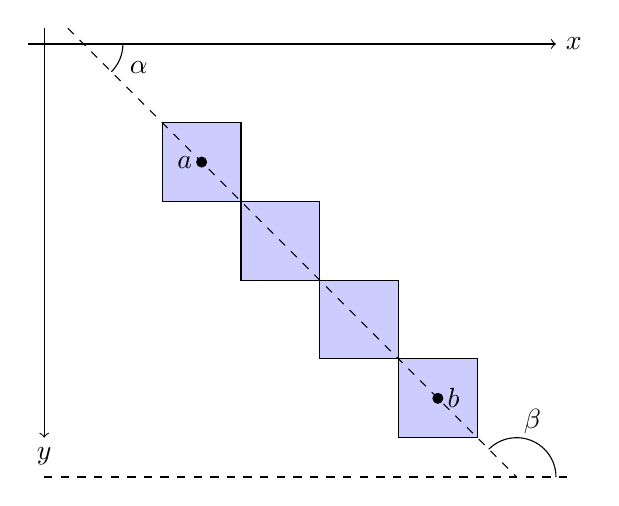
\begin{tikzpicture}
    % Draw x and y axes
    \draw[->] (0.3,0) -- (7,0) node[right] {$x$};
    \draw[->] (0.5,0.2) -- (0.5,-5) node[below] {$y$};

    % Draw the staircase
    \foreach \i in {1,...,4} {
        \draw[fill=blue!20] (\i+1,-\i) rectangle (\i+2,-\i-1);
      }

    % Draw the dashed line and the angles
    \draw[dashed] (0.8,0.2) -- (6.5,-5.5);
    \draw[dashed] (0.5,-5.5) -- (7.2,-5.5);

    \draw[-] (1.5,0) arc[start angle=0,end angle=-45,radius=0.5];
    \node at (1.7,-0.3) {$\alpha$};

    \draw[-] (7,-5.5) arc[start angle=0,end angle=135,radius=0.5];
    \node at (6.7,-4.8) {$\beta$};

    \coordinate (a) at (2.5, -1.5);
    \coordinate (b) at (5.5, -4.5);
    % Add labels
    \node at (a) [left] {$a$};
    \node at (b) [right] {$b$};

    \foreach \point in {a,b}
    \fill [black,opacity=1] (\point) circle (2pt);
  \end{tikzpicture}
  \caption {Calcolo dell'orientamento del segmento}
\end{figure}
\noindent
Inoltre, $\alpha$ è positivo in verso orario e negativo in verso antiorario. In quest'ultimo caso, l'angolo finale viene calcolato come $\theta = -\alpha$.
\begin{equation}
  \theta = \begin{cases}
    \pi - \alpha & \text{se } y_a < y_b \land x_a < x_b \\
    -\alpha      & \text{altrimenti}
  \end{cases}
\end{equation}
\subsubsection{Ricerca degli intersection points}

\subsection{Analisi dello spazio occupato}
Voronoi, trasformata skeleton
\subsubsection{Ricerca degli endpoints}

\subsection{Ricerca delle porte}

\subsection{Generazione Grafo delle Stanze}

\section{Visualizzazione e Modifica delle Stanze}

\section{Conclusioni}